\section{II. a Electricity}

\subsection{Basics}

There are two types of charge,
    those with a positive polarity and
    those with a negative polarity.
And as acient profecies have foretold, equal charges repell each other,
    and different charges attract each other.

The most important equations, maybe ever, are the Maxwell-Equations 
    (\ref{eq:gdp:iia:maxwell_eqs})

\begin{multline} \label{eq:gdp:iia:maxwell_eqs}\\
\vec{\nabla}\cdot \vec{E} = \frac{\rho}{\varepsilon_0}\\
\vec{\nabla}\cdot \times \vec{E} = -\frac{\partial \vec{B}}{\partial t}\\
\vec{\nabla}\cdot \vec{B} = 0 \\
\\
\vec{\nabla}\cdot \times \vec{B} =
    \mu_0 \left( \vec{j} + \varepsilon_0 \frac{\partial \vec{E}}{\partial t} \right)\\
\end{multline}

When a material is rubbed by a wool or leather cloth,
    the material gets charged which leads to forces beeing at play

\subsection{Attractiona/Repulsion}

The attraction of two charges is much stronger than that of gravity.
The two particles enact an force with the same absolute value,
    the two forces have different sign.


The repulsion of same charge can be used to detect the strength of charges,
    a apparatus used to measure this is called a Electrometer
This apparatus, seen in \ref{fig:gdp:ii:a:electrometer}, charges two metallic arms with the same charge,
    both arms have the same charge,
    one arm is moveable and moves away from the other arm,
    the strength of the arm determines how far the arm is pushed.

\subsection{Quantive state of Charge}

\begin{itemize}
    \item Charges cannot be arbitrarily small 
    and has to be a integer multiple of the elemental charge ($e$).

    \item The elemental charge was determined to be $e = 1.602E-19 \text{C}$,
    where the unit $1 \text{C} = 1 \text{As}$ is Coulomb.

    \item In the table \ref{tab:gdp:ii:a:parti_cha} is a sample of charge and mass of particles.

    \item Elemental particles are only able to have a charge of $e$, $-e$, or $0$,
    where massless particles are not able to have a charge other than $0$.
    \item The charge of protons and electrons are the same

\end{itemize}


Atoms are made of electrons and are core (nucleus),
    the sum of charge of all electrons is equal to the charge of the nucleus.
The nucleus is made of protons and neutrons, 
    which are both made out of quarks.
Quarks do have a charge, 
    which is not made out of integer multiples.
Such as: 
\begin{itemize}
    \item up(u), charm(c), top(t) quarks: $q_i = \frac{2}{3}e$
    \item down(d), strange(s), bottom(b) quarks: $q_i = -\frac{1}{3}e$
\end{itemize}

These quarks are unable to appear singular,
    but only in combinations such that $\sum q_{i} = n e$,
    where $n$ is a integer and $q_i$ are the charges of the quarks of the particles.

Examples:
Proton: $2 u + 1 d \Rightarrow q_p = \left( 2\cdot \frac{2}{3} e - 1/3 e\right)= e$
Neutron: $1 u + 2d \Rightarrow q_n = \left(\frac{2}{3}3-2\cdot\frac{1}{3}e = \right)3$

In a closed system the sum of charge is a constant i.e. $\sum q_i = const.$

\subsection{Transportation of Charge}

In metalls charge is able to transfer charge freely,
    this means metalls are conductors
In other materials (such as glas) charge is bound to a location,
    despite electrostatic forces acting,
    such materials are non-conductive or isolators.

\begin{note}
Stephen Gray discovered that the human body is conductive
\end{note}

\subsection{Properties of Charge:}
\begin{itemize}
    \item Particles with mass may carry a charge.

    \item Charged particles enact forces on 

    \item Charges may be positive or negative
    \item positive and negative charges can cancel out
    \item the total charge is constant
    \item the state of charge can be transfered
    \item charge is proportinal quantized
    \item Charge is meassured in Coulomb,
        which is equivalent to ampere seconds
\end{itemize}

\subsection{Law of Coulomb}

Two charged particles can enact a force on each other,
    when observing the force several observations may be made.
\begin{enumerate}
    \item the force is proportional to the charges of the particles\\
        $F\propto q_1 \wedge F\propto q_2$

    \item the charge may be attracting or repulsing
    \item the force is dependent on the distance\\
        $F \propto \frac{1}{r^2}$
\end{enumerate}

combining these properties lead to the formula in \ref{eq:gdp:iia:law_col}

\begin{equation}
    \label{eq:gdp:iia:law_col}
    \vec{F} = k frac{q_1\cdot q_2}{\abs{\vec{r}}^2} \hat{r} 
\end{equation}

The exponent if experimentally proven to be $2$,
    with an uncertainty less than $1E-16$.
If the exponent were not excatly $2$,
    this would have some weird consequences,
    such as the field inside of a hollow sphere not disappearing and
    photons having a restmass unequal to $0$

One can try to reason that $\frac{1}{r^2}$ makes sense,
    because when viewed as rays, 
    leads to the intensity of the entire surface being constant.
Which would lead to an intensity of $I(r) = \frac{P}{A} = \frac{P}{4\pi r^2}$
and would lead to $I_1 = I_2 \frac{r_2^2}{r_1^2}$

This explanation is invalid,
    because the Coloumblaw and Gravity are \textbf{not rays}


A Comparison between gravity and coulombs law is in table \ref{tab:gdp:iia:coulomb_gravity} 
    and a list of all the fundamental forces is in table \ref{tab:gdp:iia:fund_forces}
\begin{table}
    \begin{tabularx}{1.25\textwidth}{|c | l | X|}
        \hline
        & \textbf{Coloumb} & \textbf{Gravity}\\ 
        \hline
        \textbf{Cause} & charges (pos/neg) & heavy masses \\ 
        \textbf{Direction} of fource & attracting and repulsing & always attracting \\ 
        \textbf{Strength} & Big & Small \\ 
        \textbf{proportionality of distance} &  $\frac{1}{r^2}$ & $\frac{1}{r^2}$ \\
        \textbf{quantization} & only quantized multiples of $e$ & not quantized, but mass of elemental particles equal \\ 
        \textbf{conservation} & charge & not mass but energy \\ 
        \textbf{extent of source} & charges punctiform & mass is not punctiform \\ 
        \textbf{consequences} & cohesion of the microcosm & cohesion of the macrocosm \\ 
        \hline
    \end{tabularx}
    \caption{comparison of coulomb}
    \label{tab:gdp:iia:coulomb_gravity}
\end{table}

\begin{table}
    \begin{tabularx}{\textwidth}{|c|l|c|X|}
        \hline
        \textbf{force} & \textbf{interaction} & \textbf{reach} & \textbf{strength (rel)}\\ 
        \hline
        gravity & between objects with mass & $\infty$ & $1E-22$ \\ 
        weak-foce & interaction during $\beta$-decay & $leq 1E-17$ & $1E-14$ \\ 
        coulomb force & between electrical charges & $\infty$ & $1E-2$ \\ 
        strong force & between basic building blocks & $\leq 1E-15$ & $1$\\ 
        \hline
    \end{tabularx}

    \caption{List of the fundamental forces}
    \label{tab:gdp:iia:fund_forces}
\end{table}



\begin{figure}
    \centering
    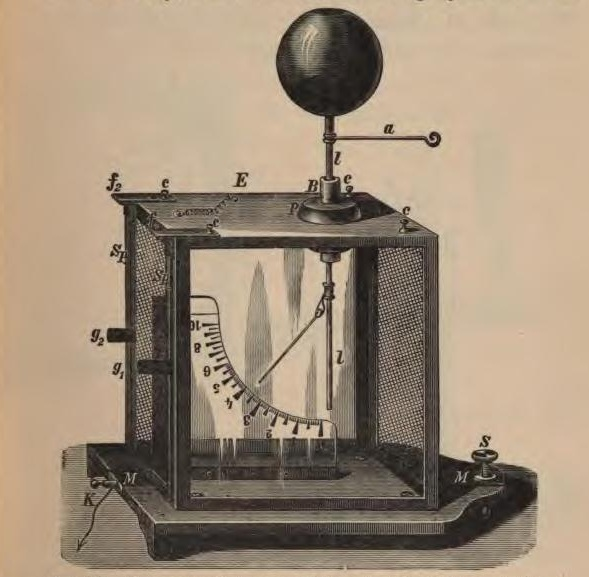
\includegraphics{gdp/ii/a/electrometer.jpg}
    \caption{Electrometer}
    \label{fig:gdp:ii:a:electrometer}
    \caption*{Source: \url{https://upload.wikimedia.org/wikipedia/commons/c/cc/\%D0\%AD\%D0\%BB\%D0\%B5\%D0\%BA\%D1\%82\%D1\%80\%D0\%BE\%D0\%BC\%D0\%B5\%D1\%82\%D1\%80_\%D0\%9A\%D0\%BE\%D0\%BB\%D1\%8C\%D0\%B1\%D0\%B5.jpg} }
\end{figure}

\begin{table}
    \begin{tabularx}{\textwidth}{c c c}
        Particle & Charge & Mass\\
        \hline
        Electron & $-e$ & $m_0$ \\
        Positron & $e$ & $m_0$ \\
        Prtoton & $e$ & $1836m_0$ \\
        Neutron & $0$ & $1836m_0$ \\
        Photon & $0$ & $0$ \\
        Neutrino & $0$ & $\geq 0$ \\
    \end{tabularx}
    \caption{charge properties of particles}
    \label{tab:gdp:ii:a:parti_cha}
\end{table}




\subsection{Electrical Field}


































